\documentclass[12pt, letterpaper, twoside]{article}    %report   ,  a4paper
\usepackage[utf8]{inputenc}
\usepackage{mathtools}
\usepackage{amsmath}
\usepackage{gensymb}

\usepackage{graphicx}
\graphicspath{ {images/} }

\title{Presek dveh implicitno danih ploskev}
\author{Matevž Vidovič}
\date{Junij, 2022}


% clicking f1 does quickbuild, which is the whole compilation at once


\begin{document}

\maketitle

$$$$

Začetne opombe: \\
- gradf1, in gradf2 vračata vrstične vektorje. \\
- testi vzamejo približno 12 sekund. \\

$$$$

\tableofcontents

\newpage



\section{Konstrukcija G in JG}
 
$$y = x + hF(x)$$
$$v = F(y)$$

\begin{equation}
\begin{split}
f_1(x) = 0 \\
f_2(x) = 0 \\
v \cdot x - v \cdot y = 0 \\
\end{split}
\end{equation}

\[
\begin{split}
h(x) = v \cdot x - v \cdot y \\
h_{x_i} = (v \cdot x)_{x_i} - (v \cdot y)_{x_i} = (v \cdot x)_{x_i} - 0 = \\
= (v_1 \cdot x_1 + v_2 \cdot x_2 + v_3 \cdot x_3)_{x_i} = v_i \\
grad h(x) = (v_1, v_2, v_3)
\end{split}
\]


\[
G(x) = 
	\begin{bmatrix}
		f_1(x) \\
		f_2(x) \\
		v \cdot x - v \cdot y		
	\end{bmatrix}
\]


\[
JG(x) = 
	\begin{bmatrix}
		grad f_1(x)_1 & grad f_1(x)_2 & grad f_1(x)_3 \\
		grad f_2(x)_1 & grad f_2(x)_2 & grad f_2(x)_3 \\
		v_1 & v_2 & v_3
	\end{bmatrix}
\]

\newpage

\section{Prevod lažjih funkcij v \\ $F(x) : R^3 \rightarrow R, F(x) = 0$:}

Prevod enačbe ravnine na $F(x)=0$: \\
$$n \cdot x = n \cdot r$$
$$n \cdot x - n \cdot r = 0$$
$$F(x) = n \cdot x - n \cdot r$$
n je normalni vektor ravnine, r je krajevni vektor ene točke na ravnini.

$$$$

Prevod iz $f(x) : R^2 \rightarrow R$ na $F(x)=0$: \\
Ravnina $x_1, x_3$ je domena funkcije. \\
$x_2$ predstavlja vrednost $f(x_1, x_3)$ \\
$x_2$ si predstavljam kot vertikalno dimenzijo. \\
$$x_2 = f(x_1, x_3)$$
$$0 = f(x_1, x_3) - x_2$$
$$F(x_1, x_2, x_3) := f(x_1, x_3) - x_2$$
$$ \Rightarrow F(x) = 0 \Leftrightarrow x_2 = f(x_1, x_3)$$

\newpage

\section{Testi}

$$$$

Test 1:

\begin{equation}
\begin{split}
n_1 = [1, 1, 0]^T \\
n_2 = [-1, 1, 0]^T \\
r_{1, 2} = [0, 0, 0]^T \\
F_1(x) = x_1 + x_2 \\
F_2(x) = -x_1 + x_2 \\
\end{split}
\end{equation}
Presek bo premica [0, 0, r]; r e R

$$$$

Test 2:
\begin{equation}
\begin{split}
n_1 = [1, 1, 0]^T \\
n_2 = [-1, 1, 0]^T \\
r_{1, 2} = [1, 0, 0]^T \\
F_1(x) = x_1 + x_2 - 1 \\
F_2(x) = -x_1 + x_2 + 1\\
\end{split}
\end{equation}
Presek bo premica [1, 0, r]; r e R

$$$$

Test 3:
\begin{equation}
\begin{split}
f(x_1, x_3) = x_1^2 + x_3^2 \\
F_1(x) = x_1^2 + x_3^2 - x_2 \\
\\
x_1^2 + x_3^2 = C = x_2 \\
x^2 + y^2 = (r^2) \Rightarrow krog \\
\Rightarrow r = \sqrt{C} = \sqrt{x_2} = \sqrt{n_2 \cdot r_2} \\
\\
n_2 = [0, 1, 0]^T \\
r_2 = [0, 5, 0]^T \\
F_2(x) = x_2 - 5\\
\end{split}
\end{equation}
Če gledamo preseke z $x_1, x_3$ ravnino, dobimo krožnice.
To lahko vidimo, če pogledamo, kdaj ima funkcija $f(x)$ neko konstantno vrednost. \\
Ravnina $F_2(x)$ je vzporedna ravnini $x_1, x_3$, saj imata obe normalni vektor $[0, 1, 0]^T$.
Iz enačbe $F_2(x) = 0$ pa vidimo, da je $x_2$ ravno $n_2 \cdot r_2$. \\
Za našo krivuljo bo torej veljalo, da je skupina vektorjev, kjer veljata enačbi $x_1^2 + x_3^2 = n_2 \cdot r_2$ in $x_2 = n_2 \cdot r_2$ \\

$$$$
$$$$

Test 4:
\begin{equation}
\begin{split}
f(x_1, x_3) = (\frac{x_1}{2})^2 + (\frac{x_3}{5})^2 \\
F_1(x) = (\frac{x_1}{2})^2 + (\frac{x_3}{5})^2 - x_2 \\
\\
(\frac{x_1}{2})^2 + (\frac{x_3}{5})^2 = C = x_2 \\
(\frac{x}{a})^2 + (\frac{y}{b})^2 = C \Rightarrow elipsa \\
\\
n_2 = [0, 1, 0]^T \\
r_2 = [0, 7, 0]^T \\
F_2(x) = x_2 - 7
\end{split}
\end{equation}
Če gledamo preseke z $x_1, x_3$ ravnino, dobimo elipse.
To lahko vidimo, če pogledamo, kdaj ima funkcija $f(x)$ neko konstantno vrednost. \\
Ravnina $F_2(x)$ je vzporedna ravnini $x_1, x_3$, saj imata obe normalni vektor $[0, 1, 0]^T$.
Iz enačbe $F_2(x) = 0$ pa vidimo, da je $x_2$ ravno $n_2 \cdot r_2$. \\
Za našo krivuljo bo torej veljalo, da je skupina vektorjev, kjer veljata enačbi $(\frac{x_1}{2})^2 + (\frac{x_3}{5})^2 = n_2 \cdot r_2$ in $x_2 = n_2 \cdot r_2$ \\

$$$$
$$$$

Test 5: isti primer kot test 4, le da bo C oziroma $x_2$ enak 1. \\
Tako je graf bolj pregleden, saj se točno vidi polosi.
\begin{equation}
\begin{split}
f(x_1, x_3) = (\frac{x_1}{2})^2 + (\frac{x_3}{5})^2 \\
F_1(x) = (\frac{x_1}{2})^2 + (\frac{x_3}{5})^2 - x_2 \\
\\
n_2 = [0, 1, 0]^T \\
r_2 = [0, 1, 0]^T \\
F_2(x) = x_2 - 1
\end{split}
\end{equation}

$$$$
$$$$

Test 6: Normalni vektor ravnine je $45\degree$ glede na $x_2, x_3$ ravnino.
Torej bo $F_2(x)$ glede na ravnino $x_2, x_3$ ravno $-45\degree$.
\begin{equation}
\begin{split}
f(x_1, x_3) = (\frac{x_1}{2})^2 + (\frac{x_3}{5})^2 \\
F_1(x) = (\frac{x_1}{2})^2 + (\frac{x_3}{5})^2 - x_2 \\
\\
n_2 = [0, 1, 1]^T \\
r_2 = [0, 5, 0]^T \\
F_2(x) = x_2 + x_3 - 5 \\
\\
F_2(x) = 0 \\
x_2 = - x_3 + 5 \\
F_1(x) = 0 \\
(\frac{x_1}{2})^2 + (\frac{x_3}{5})^2 = x_2 \\ 
\\
Krivulja \Leftrightarrow (\frac{x_1}{2})^2 + (\frac{x_3}{5})^2 = - x_3 + 5 \\
\end{split}
\end{equation}
$$$$

\newpage

\section{Koda za grafe testov}
Test 1: \\
F1 = @(X) (X(1) + X(2)); \\
F2 = @(X) (-X(1) + X(2)); \\
gradF1 = @(X) ([1, 1, 0]); \\
gradF2 = @(X) ([-1, 1, 0]); \\
Y = presekPloskev(F1, gradF1, F2, gradF2, [0.01; 0.02; 0.4], 0.1, 300, 1e-10, 100); \\
plot3(Y(1, : ), Y(3, : ), Y(2, : )); \\
axis equal; \\
xlabel ("x1"); \\
ylabel ("x3"); \\
zlabel("x2"); \\

$$$$

Test 2: \\
F1 = @(X) (X(1) + X(2) - 1); \\
F2 = @(X) (-X(1) + X(2) + 1); \\
gradF1 = @(X) ([1, 1, 0]); \\
gradF2 = @(X) ([-1, 1, 0]); \\
Y = presekPloskev(F1, gradF1, F2, gradF2, [0.01; 0.02; 0.4], 0.1, 300, 1e-10, 100); \\
plot3(Y(1, : ), Y(3, : ), Y(2, : )); \\
axis equal; \\
xlabel ("x1"); \\
ylabel ("x3"); \\
zlabel("x2"); \\

\newpage

Test 3: \\
F1 = @(X) (X(1)\^{}2 + X(3)\^{}2 - X(2)); \\
F2 = @(X) (X(2) - 5); \\
gradF1 = @(X) ([2*X(1), -1, 2*X(3)]); \\
gradF2 = @(X) ([0, 1, 0]); \\
Y = presekPloskev(F1, gradF1, F2, gradF2, [0.8; 0.8; 0.2], 0.1, 300, 1e-10, 100); \\
plot3(Y(1, : ), Y(3, : ), Y(2, : )); \\
axis equal; \\
xlabel ("x1"); \\
ylabel ("x3"); \\
zlabel("x2"); \\

$$$$

Test 4: \\
F1 = @(X) ((X(1)/2)\^{}2 + (X(3)/5)\^{}2 - X(2)); \\
F2 = @(X) (X(2) - 7); \\
gradF1 = @(X) ([X(1)/2, -1, 2*X(3)/25]); \\
gradF2 = @(X) ([0, 1, 0]); \\
Y = presekPloskev(F1, gradF1, F2, gradF2, [0.8; 0.8; 0.2], 0.1, 700, 1e-10, 100); \\
plot3(Y(1, : ), Y(3, : ), Y(2, : )); \\
axis equal; \\
xlabel ("x1"); \\
ylabel ("x3"); \\
zlabel("x2"); \\

\newpage

Test 5: \\
F1 = @(X) ((X(1)/2)\^{}2 + (X(3)/5)\^{}2 - X(2)); \\
F2 = @(X) (X(2) - 1); \\ 
gradF1 = @(X) ([X(1)/2, -1, 2*X(3)/25]); \\
gradF2 = @(X) ([0, 1, 0]); \\
Y = presekPloskev(F1, gradF1, F2, gradF2, [0.8; 0.8; 0.2], 0.1, 300, 1e-10, 100); \\
plot3(Y(1, : ), Y(3, : ), Y(2, : )); \\
axis equal; \\
xlabel ("x1"); \\
ylabel ("x3"); \\
zlabel("x2"); \\

$$$$

Test 6: \\
F1 = @(X) ((X(1)/2)\^{}2 + (X(3)/5)\^{}2 - X(2)); \\
F2 = @(X) (X(2) +  X(3) - 5); \\
gradF1 = @(X) ([X(1)/2, -1, 2*X(3)/25]); \\
gradF2 = @(X) ([0, 1, 1]); \\
Y = presekPloskev(F1, gradF1, F2, gradF2, [0.8; 0.8; 0.2], 0.1, 1200, 1e-10, 100); \\
plot3(Y(1, : ), Y(3, : ), Y(2, : )); \\
axis equal; \\
xlabel ("x1"); \\
ylabel ("x3"); \\
zlabel("x2"); \\

\newpage

\section{Slike testov}
Test 1: \\
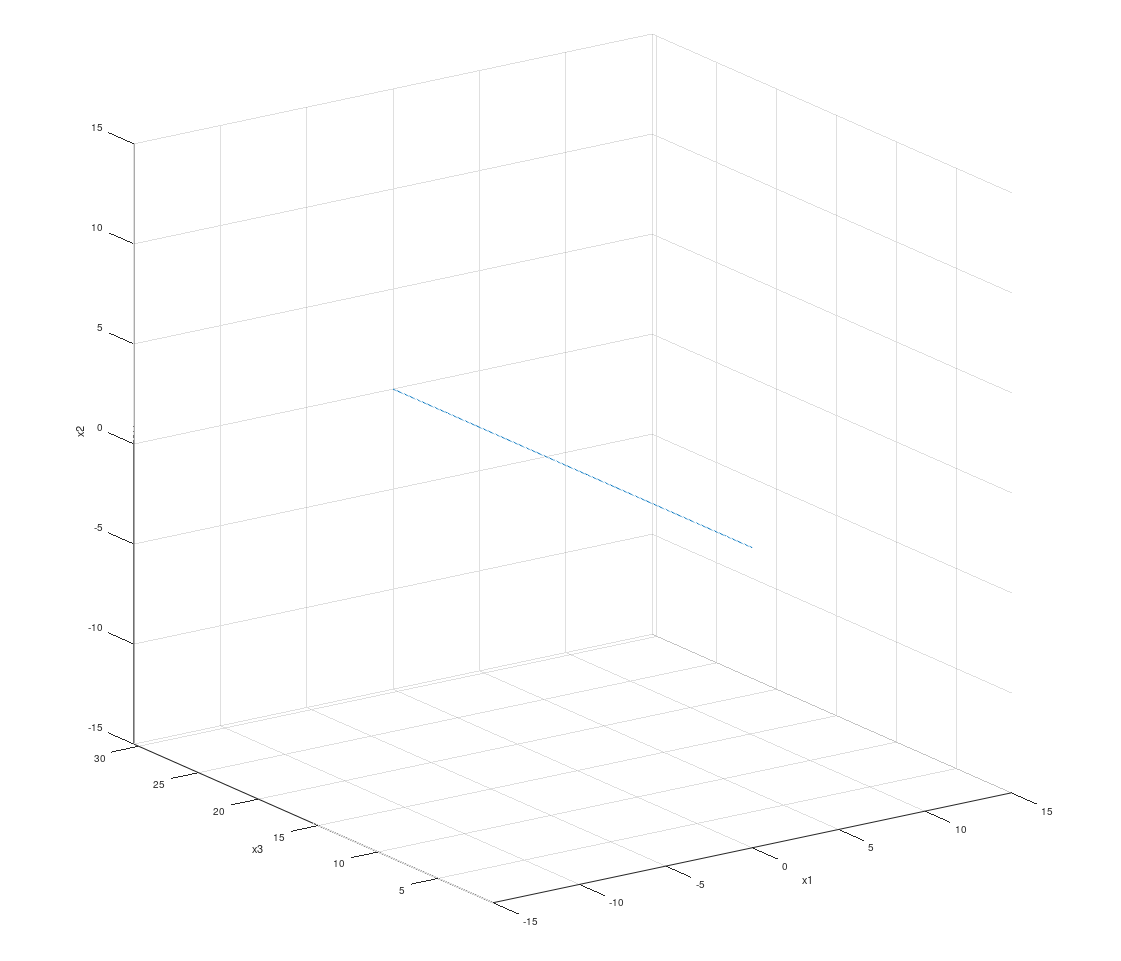
\includegraphics[width=\textwidth]{test1}
\newpage
Test 2: \\
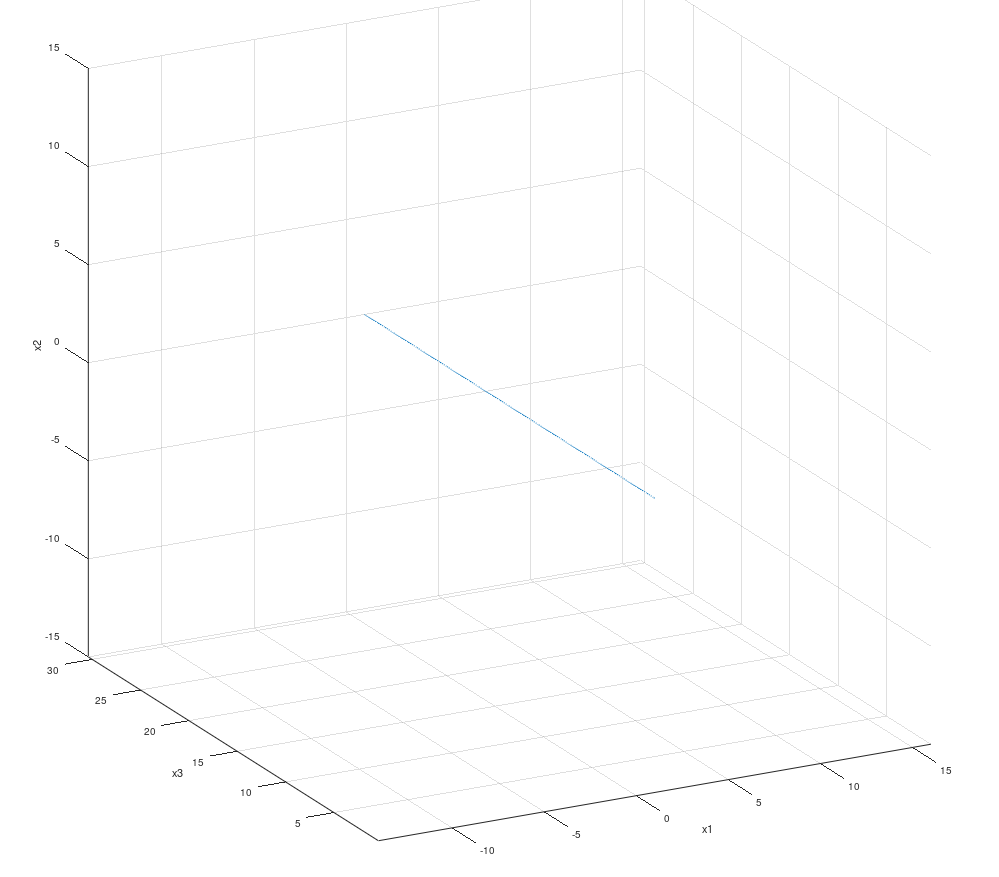
\includegraphics[width=\textwidth]{test2}
\newpage
Test 3: \\
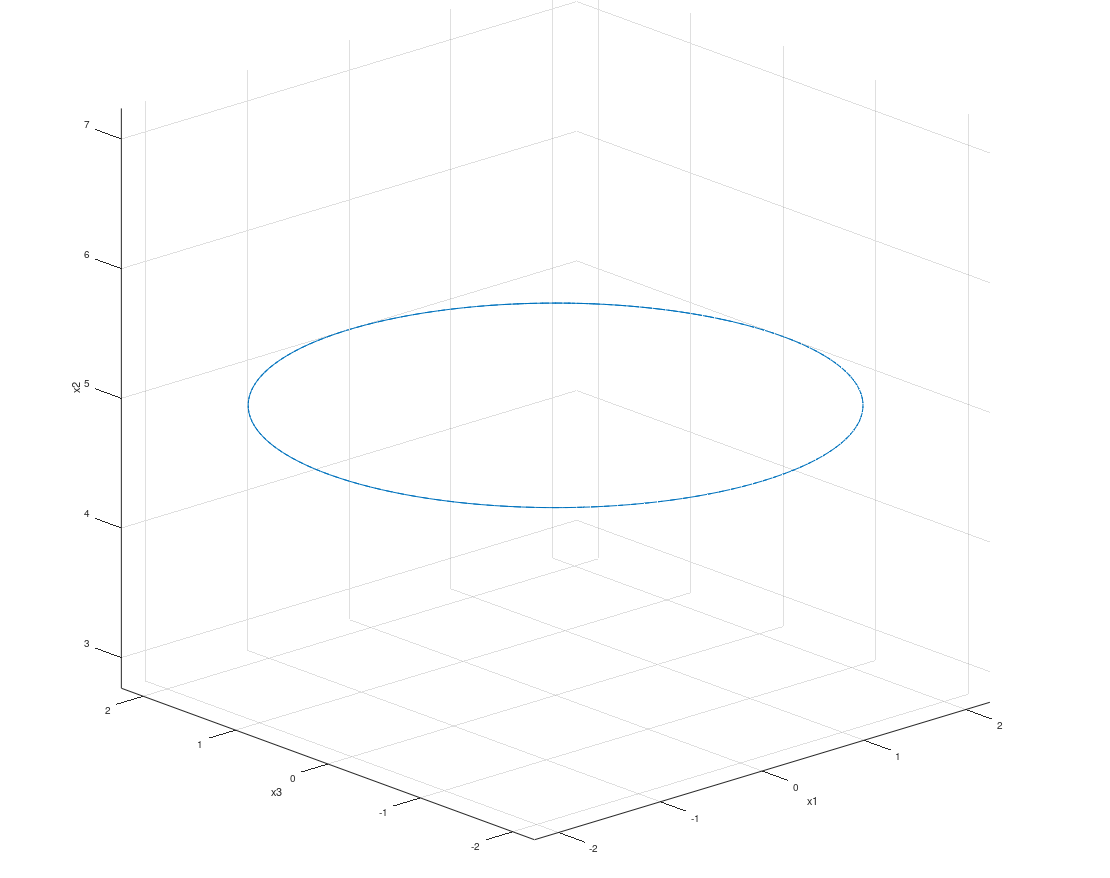
\includegraphics[width=\textwidth]{test31}
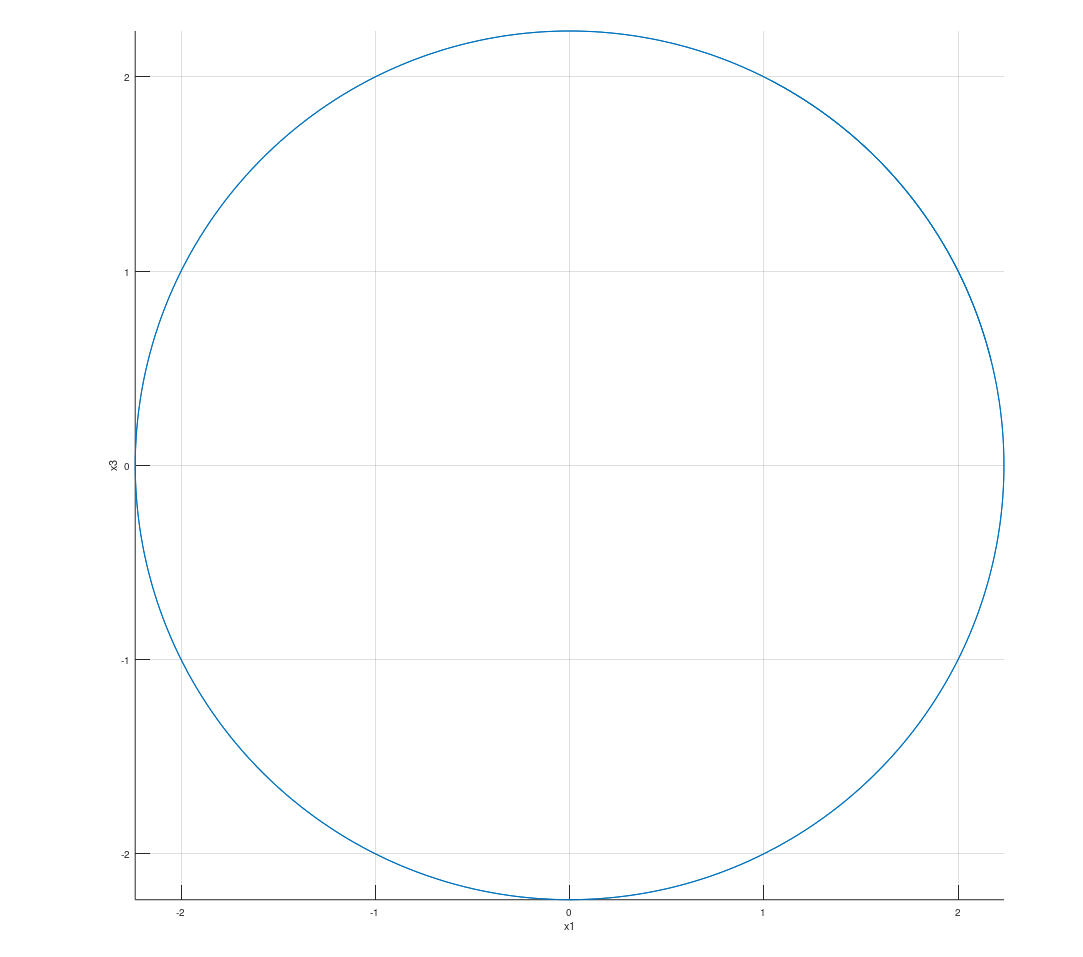
\includegraphics[width=\textwidth]{test32}
\newpage
Test 4: \\
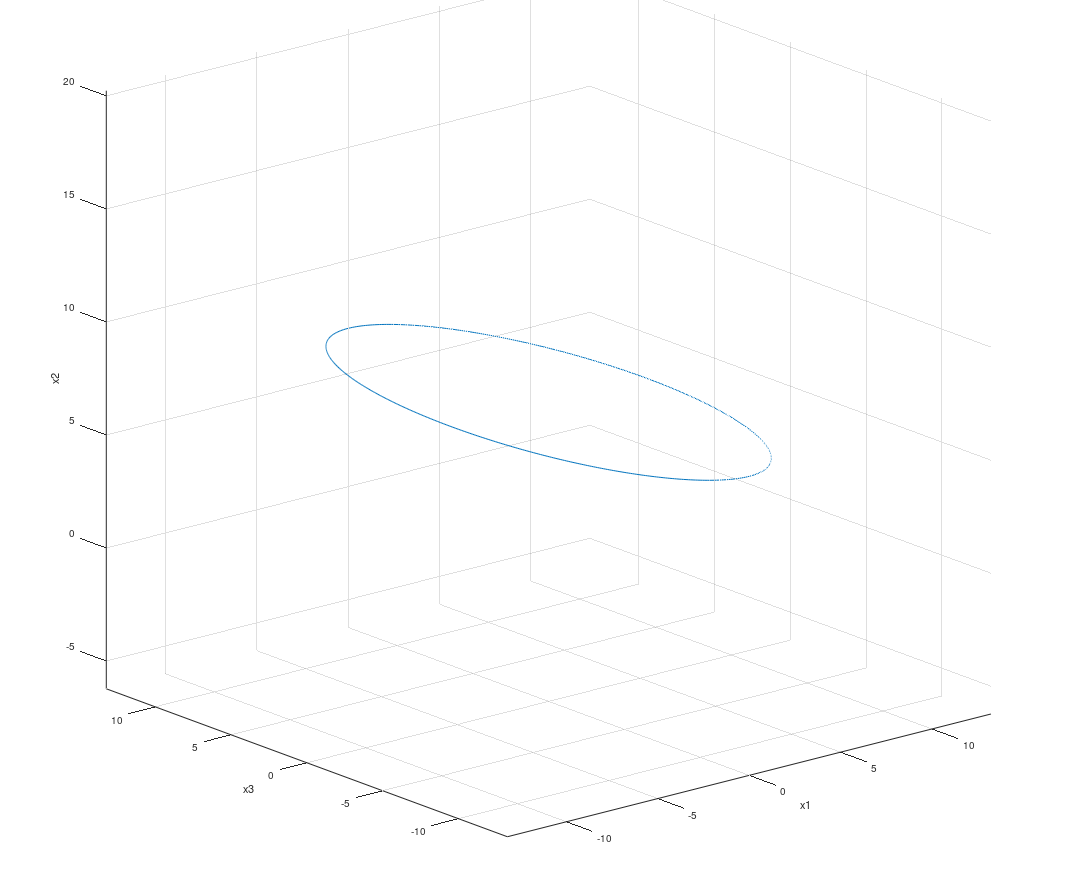
\includegraphics[width=\textwidth]{test41}
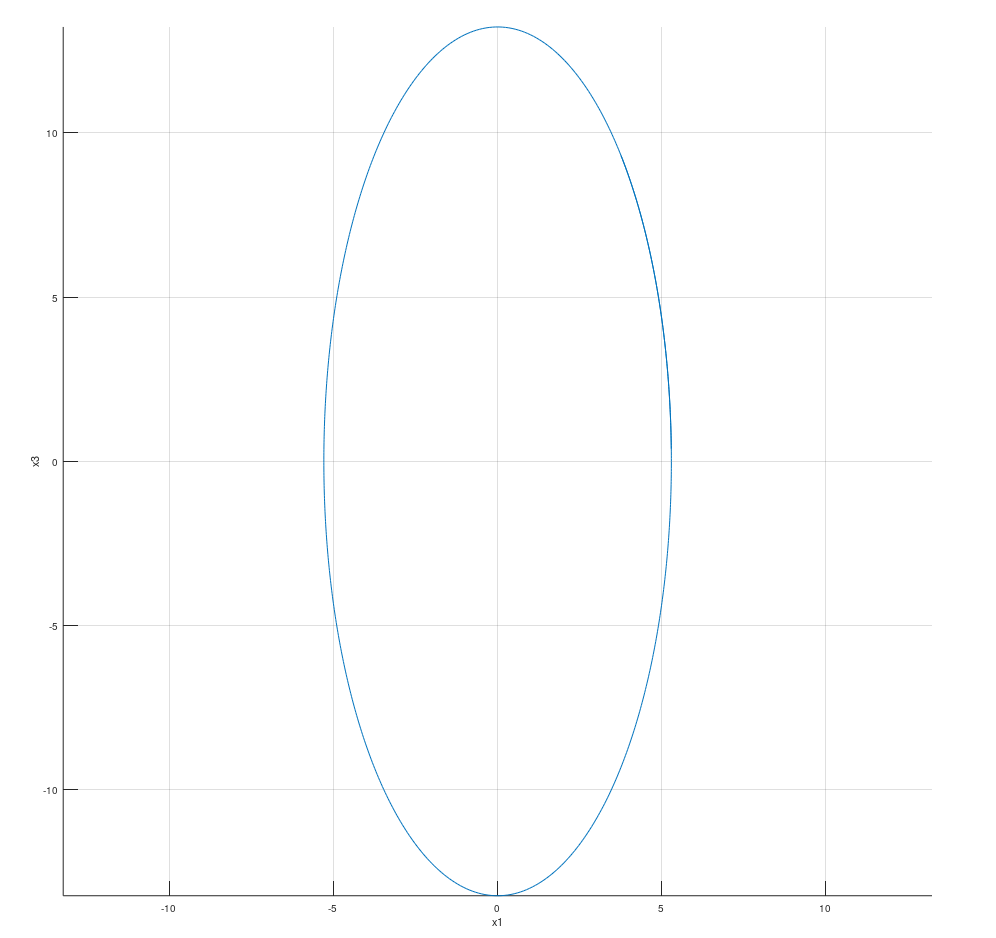
\includegraphics[width=\textwidth]{test42}
\newpage
Test 5: \\
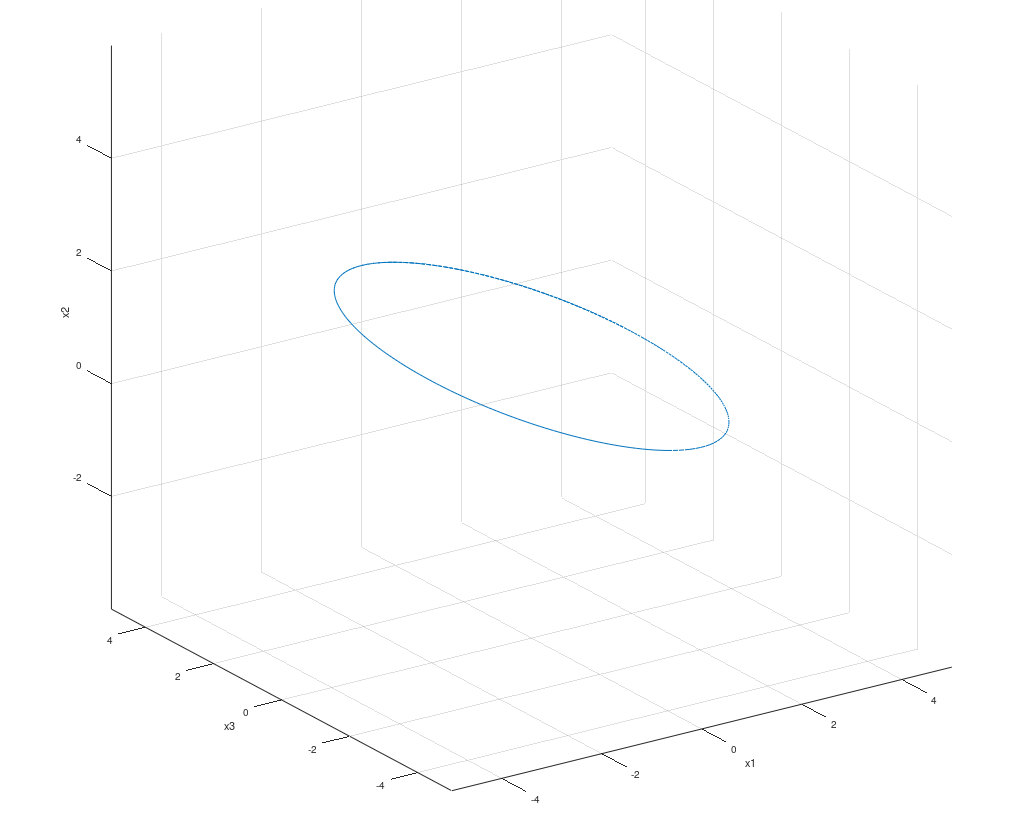
\includegraphics[width=\textwidth]{test51}
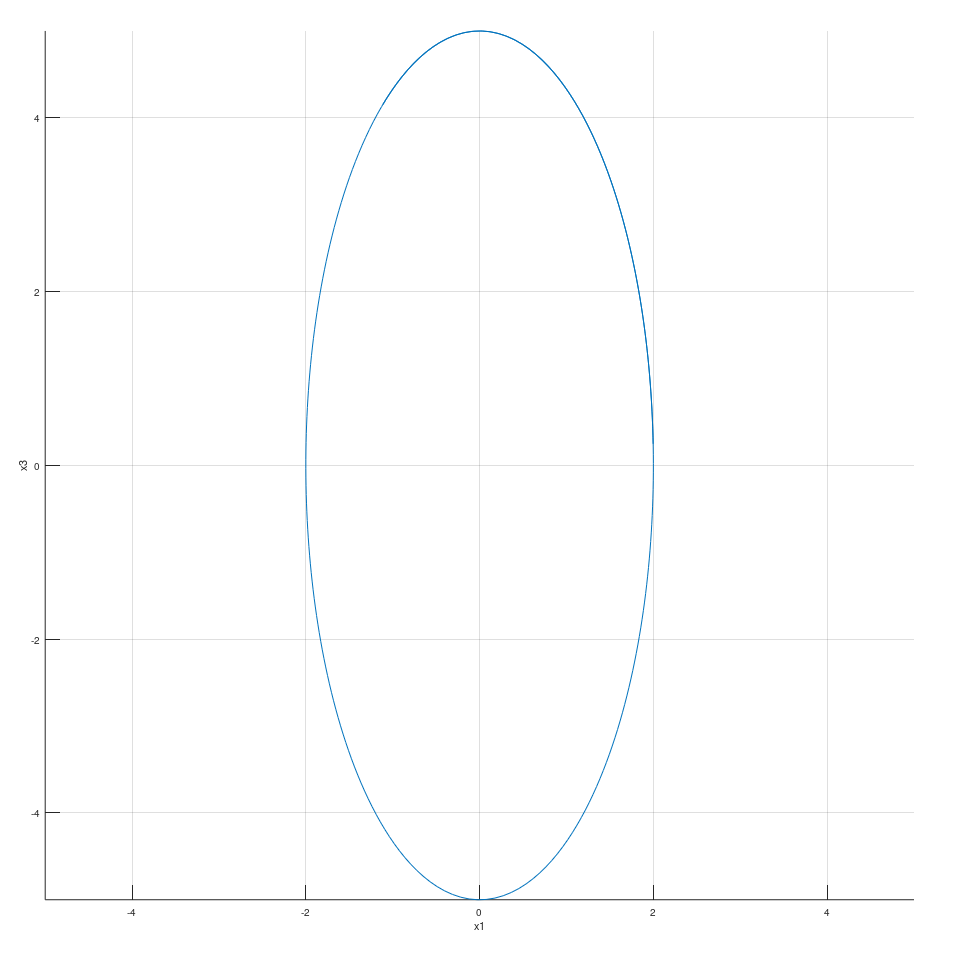
\includegraphics[width=\textwidth]{test52}
\newpage
Test 6: \\
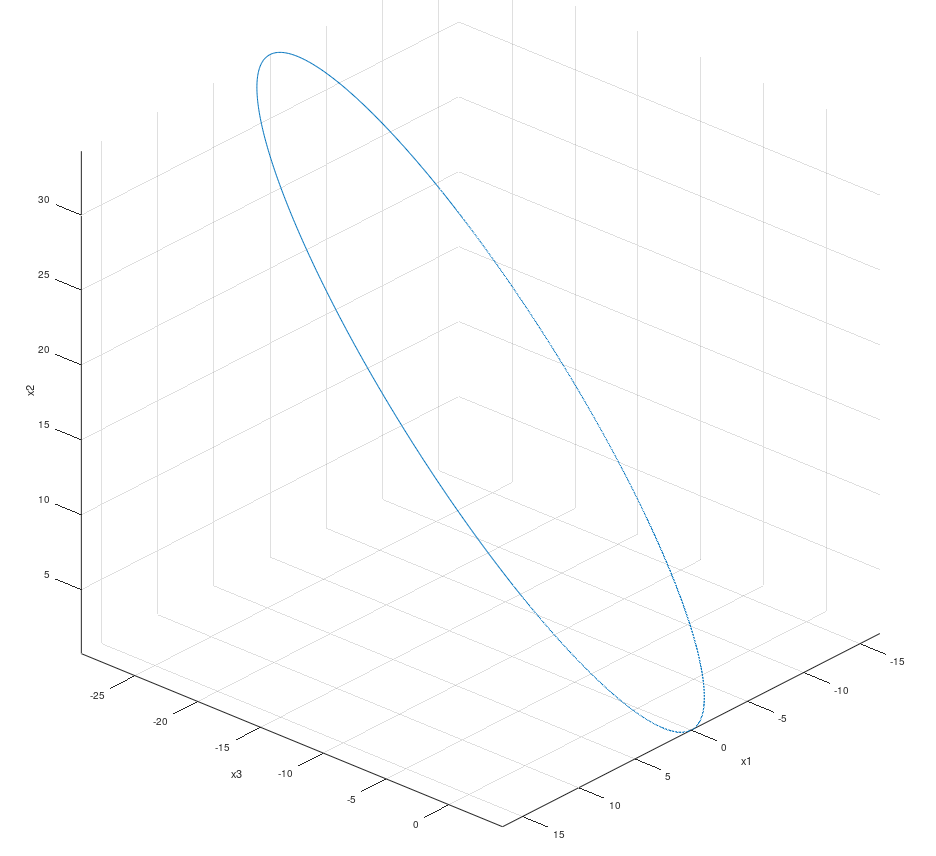
\includegraphics[width=\textwidth]{test61}
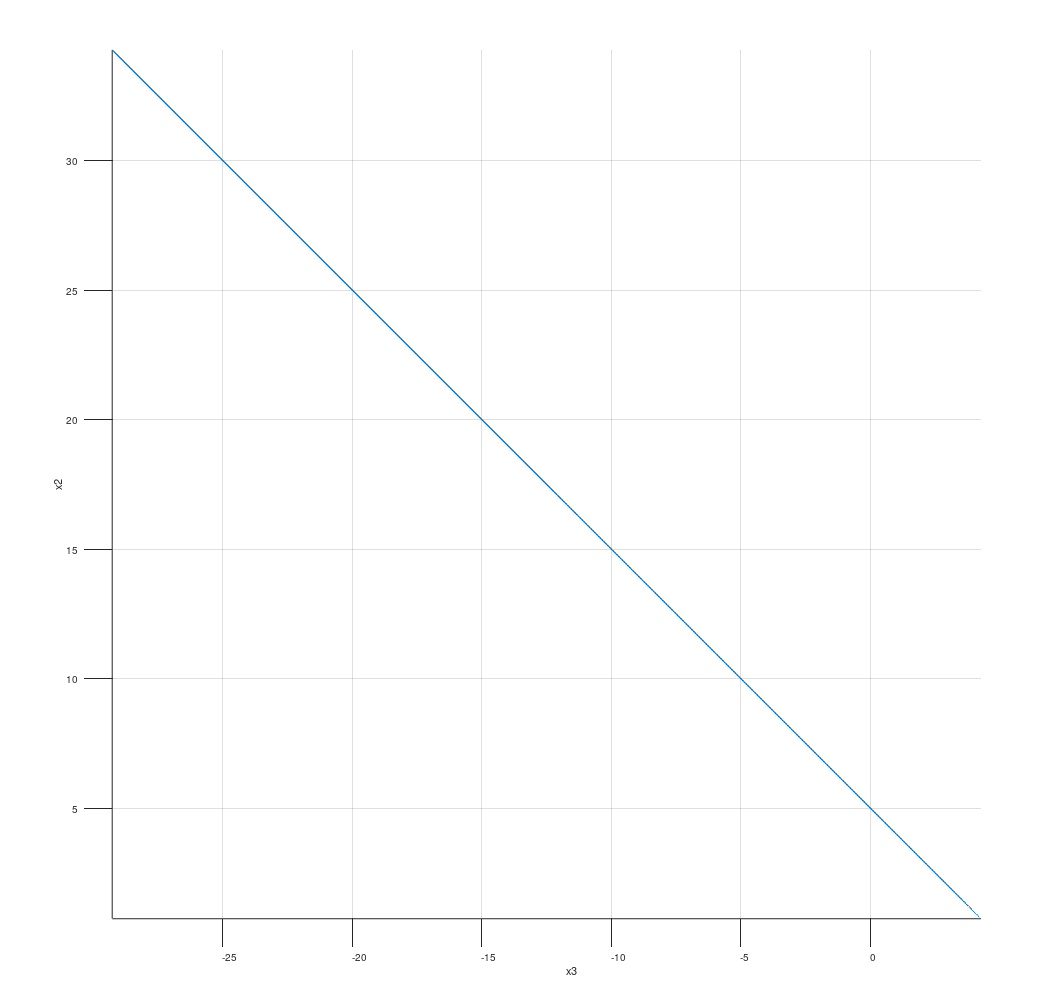
\includegraphics[width=\textwidth]{test62}
\newpage






\end{document}